\documentclass[a4paper]{report}


\usepackage{titlesec}
\usepackage{lipsum}
\usepackage{ifdraft}
\usepackage{amsmath}
\usepackage{amsfonts}
\usepackage{amssymb}
\usepackage{natbib}
\usepackage{rotating}
\usepackage{hyperref}
\usepackage{subfig} 
\usepackage{appendix}
\usepackage{tipa}
\usepackage{clrscode}
\usepackage{setspace}
\usepackage{graphicx}
\usepackage[absolute]{textpos} 
\usepackage[top=1in, bottom=1in, left=1in, right=1in, paperwidth=8.5in, paperheight=11in]{geometry}

\titleformat{\chapter}
  {\normalfont\bfseries}{}{0pt}{\Large}
  
\begin{document}

\setlength{\TPHorizModule}{200mm} 
\setlength{\TPVertModule}{100mm} 
\textblockorigin{61mm}{19mm}


 

% activate for ONSCREEN reading shape AT HOME
%\usepackage[top=0.1in, bottom=0.1in, left=0.3in, right=0.3in, paperwidth=11in, paperheight=8.5in]{geometry} % activate for ONSCREEN reading shape AT WORK

\onehalfspace{}

% activate the appropriate shortcut, whether or not to show this in titles
%	\providecommand{\doneit}{DONE: }
%	\providecommand{\doneit}{}


% numbering starts from here:
\pagenumbering{arabic}

% titlepage stuff
\title{\textbf{Introduction to RStudio for Windows}}
\author{Center for Interdisciplinary Research and Consulting
\\
Department of Mathematics and Statistics
\\
University of Maryland, Baltimore County
\\
http://www.umbc.edu/circ/
}

\date{2019}

\maketitle
\newpage
\section*{About Us}
    \begin{flushleft}
        The Center for Interdisciplinary Research and Consulting (CIRC) is a consulting service on mathematics and statistics provided by the Department of Mathematics and Statistics at UMBC. Established in 2003, we provide a full range of consulting services on Mathematics and Statistics in broad areas of applications, including biological sciences, engineering, and social sciences to the UMBC community and public. 
    \end{flushleft}

    \begin{flushleft}
        We can also provide service with software packages such as SAS, SPSS, and S-Plus, MATLAB AND FEMLAB.
    \end{flushleft}

\section*{Contact Us}
    \begin{flushleft}
        Center for Interdisciplinary Research and Consulting (CIRC)
 
        \newline Department of Mathematics and Statistics

        \newline University of Maryland, Baltimore County

        \newline 1000 Hilltop Circle
Baltimore, MD 21250

        \newline U.S.A.
        \end{flushleft}
        
        \begin{flushleft}
        Math/Psyc Building, Room 422A

        \newline Phone: (410) 455-2409

        \newline Fax: (410) 455-1066

        \newline E-mail: circ@umbc.edu
    \end{flushleft}

\setcounter{page}{2}
\tableofcontents
\chapter{1 - Introduction}
    \section{What is R?}
    
        \begin{flushleft}
        R is a statistical software system for data analysis and graphics developed by Ross Ihaka and Robert Gentlemen of the Statistics Department of the University of Auckland in 1995. R is considered as a dialect of the language S and S-Plus created by Bill Venables and David M. Smith (Insightful Corporation). R is currently developed by the R core-development team.
        \end{flushleft}
        
        \begin{flushleft}
        R is an object-oriented language. This means that everything in R is stored in active memory of the computer in the form of object. We can edit objects and do actions on objects with operators.
        \end{flushleft}
        
    \section{What is RStudio?}
    
        \begin{flushleft}
       RStudio is an integrated development environment (IDE) for R, which allows the user to run R in a more user-friendly environment. It was created by J.J. Allaire in 2008, supported by Foundation for Open Access Statistics (FOAS) and R Consortium. RStudio can be run on the desktop (Windows, Mac and Linux) or it can be accessed in a browser connected to the RStudio Server.
        \end{flushleft}
        
    \section{Why RStudio?}
    
        \begin{flushleft}
        The goal of the present document is to be an introduction of RStudio for beginners.  RStudio is available in open source and commercial editions and can be run on various platforms such as Unix, Windows and Mac. One of the benefits of using RStudio, besides it's user-friendly environment, is that it looks and feels the same regardless of the platform. The environment makes accessing and employing the many built-in functions for statistical analysis that R has simple and can produce excellent graphics. R language is easy to combine with other user-written functions. Also, R can handle much larger datasets compared to S-Plus.
        \end{flushleft}
    
    \newpage 
    
    \section{Where can I get RStudio?}
       \begin{flushleft}
            RStudio is available in an open source edition and is available for Unix, Windows and Mac. This document provides installation instructions for Windows; however, the installation on other operating systems is similar. 
            
          \textbf{Step-1:} \textbf{https://www.rstudio.com/products/rstudio/download/}
          
          \textbf{Step-2:} Under the "RStudio Desktop Open Source License" tab, click download. 
          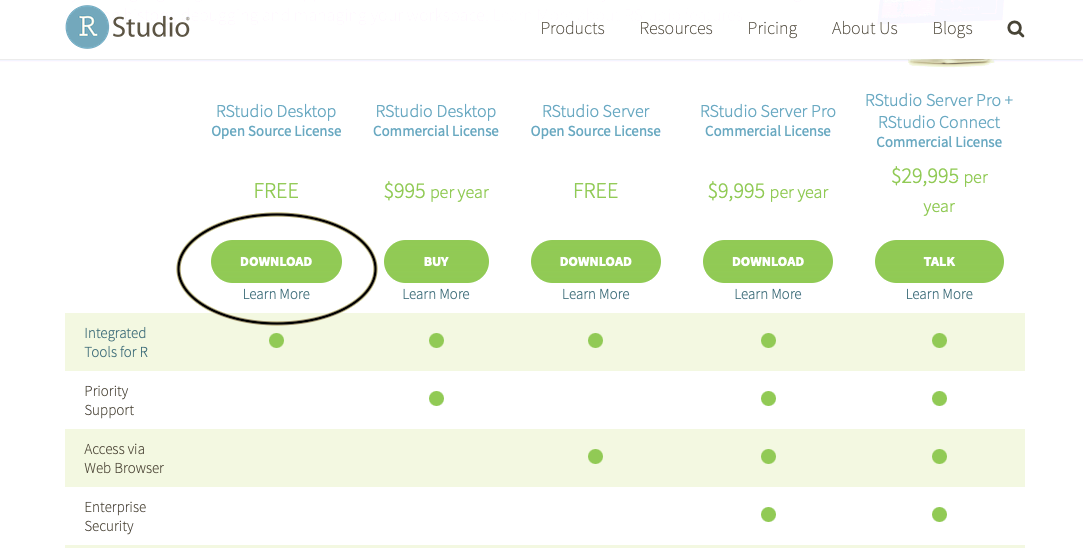
\includegraphics[width=\textwidth]{images/download1.png}
          
         \textbf{Step-3:}Click on the RStudio installer for Windows, and save the setup file in your local directory. 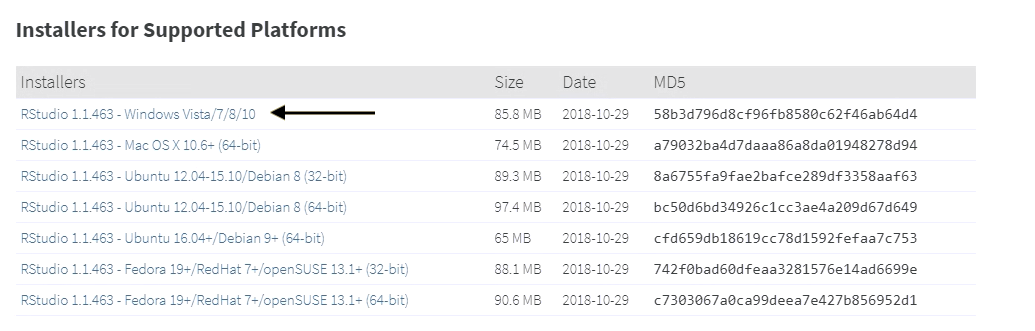
\includegraphics[width=\textwidth]{images/download2.png}
         
         \newpage
         
        \textbf{Step-4:} Run the RStudio installer. 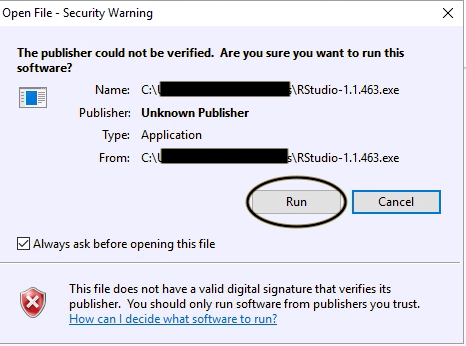
\includegraphics[width=\textwidth]{images/download3.png}

      \end{flushleft}

       
      
    
    \section{Reference}
    Online R tutorial. \underline{"http://cran.r-project.org/doc/manuals/R-intro.html#References"}

\chapter{2 - Getting Started}

    \section{Opening RStudio}
        \begin{flushleft}
        In windows, the easiest way to open RStudio is by accessing it through the start menu. 
        \newline
        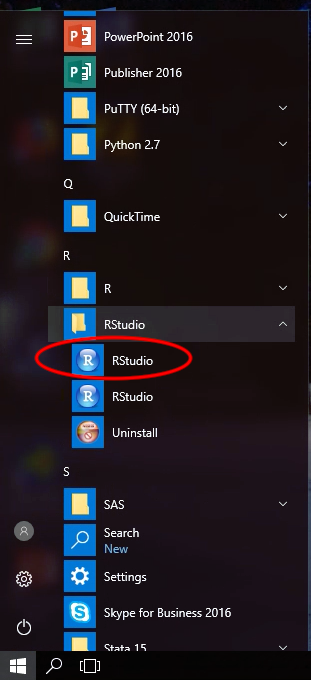
\includegraphics[width=3.5in, height=6in]{images/GS1.png}
        \end{flushleft}
    \section{The RStudio Interface}

        \begin{flushleft}
            RStudio has four panes in the interface that are the most important. The first is the R script window or Source Editor, this is located in the top left of the RStudio window and does not open automatically when you initially open RStudio. This is where most programs will be written, we will see how to create and save an R script file in a later section.  
            \newline \newline
            The second is the RStudio Console window. In the RStudio Console Window, you must execute each line one step at a time. Also, when you exit the current RStudio session,these commands will be lost. 
            \newline \newline
            The third is the Environment and History window located on the top right of the RStudio window. Environment pane shows all the active objects. The history pane shows a list of commands used so far 
            \newline \newline
            The last is the Files, Plots, Packages, Help and Viewer window located on the bottom right of the RStudio window. This is where you can search, load and install packages (which will be discussed in a later section), view plots, view and open files, get help on functions and packages as well as viewing local web content. 
             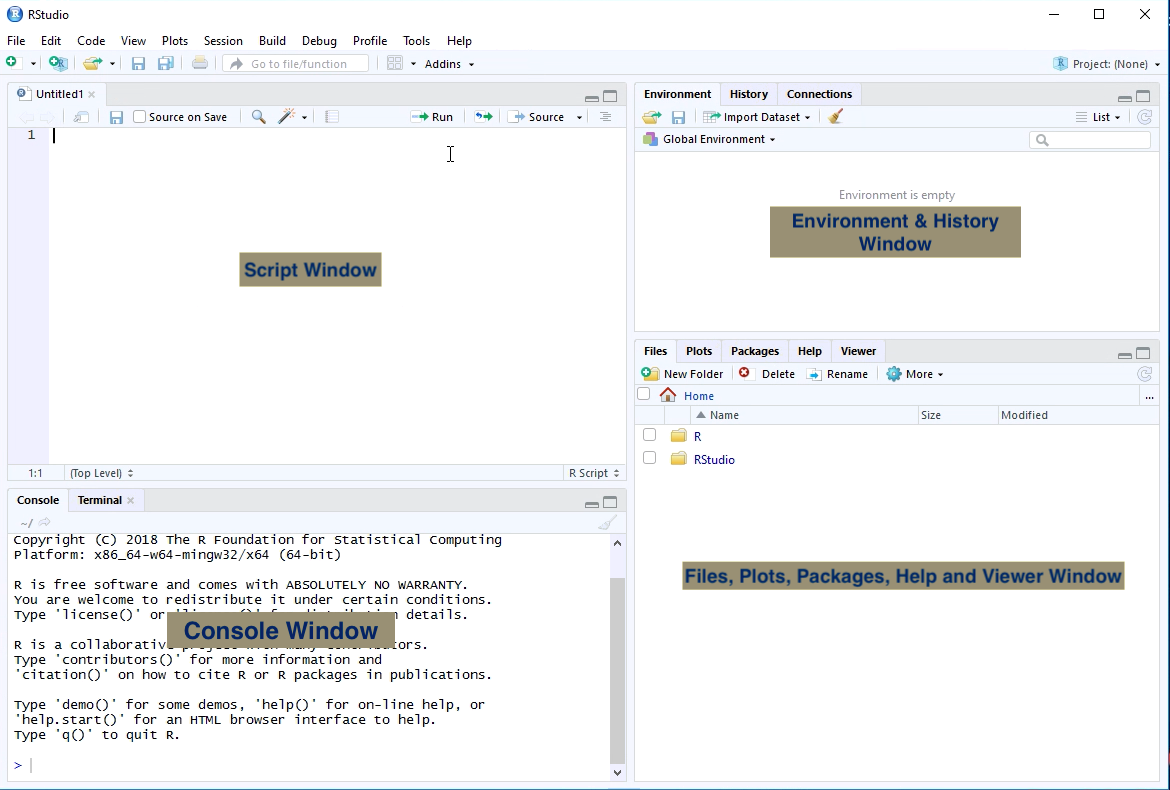
\includegraphics[width=\textwidth]{images/GS4.png}
        \end{flushleft}
       
   \newpage \section{Closing RStudio}
    
        \begin{flushleft}
            You can exit Rstudio from either the file menu, by selecting File $\longrightarrow \textbf{Exit}$ or type the command in RStudio Console Window: ``q()"
           
         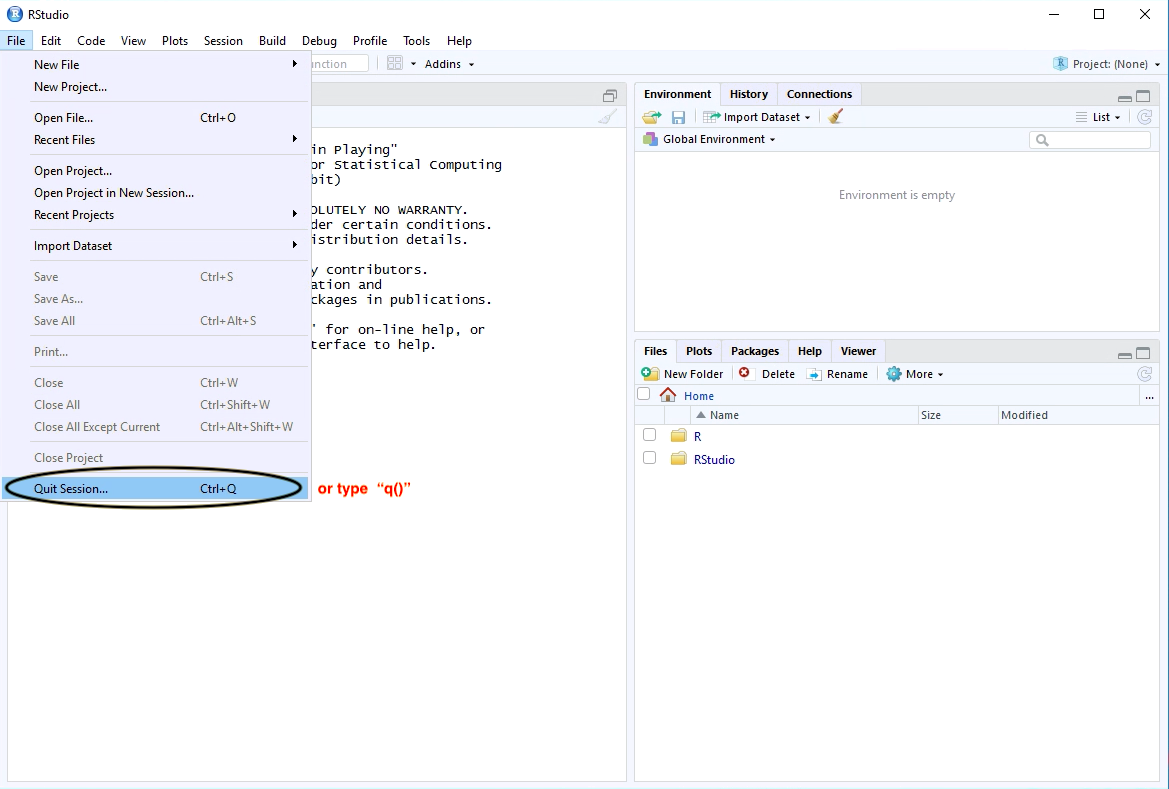
\includegraphics[width=\textwidth]{images/GS3.png}
        \end{flushleft}
        
    \newpage \section{Using Help in RStudio}
        \begin{flushleft}
        One of the many advantages of using RStudio is how easy it makes it to get help on functions and packages. There are many ways to do this. 
        \newline \newline 
        The first way is to use the ``Help" tab in the Files, Plots, Packages, Help and Viewer pane. When you click the ``Help" tab, you will see links to helpful resources about R and RStudio. 
        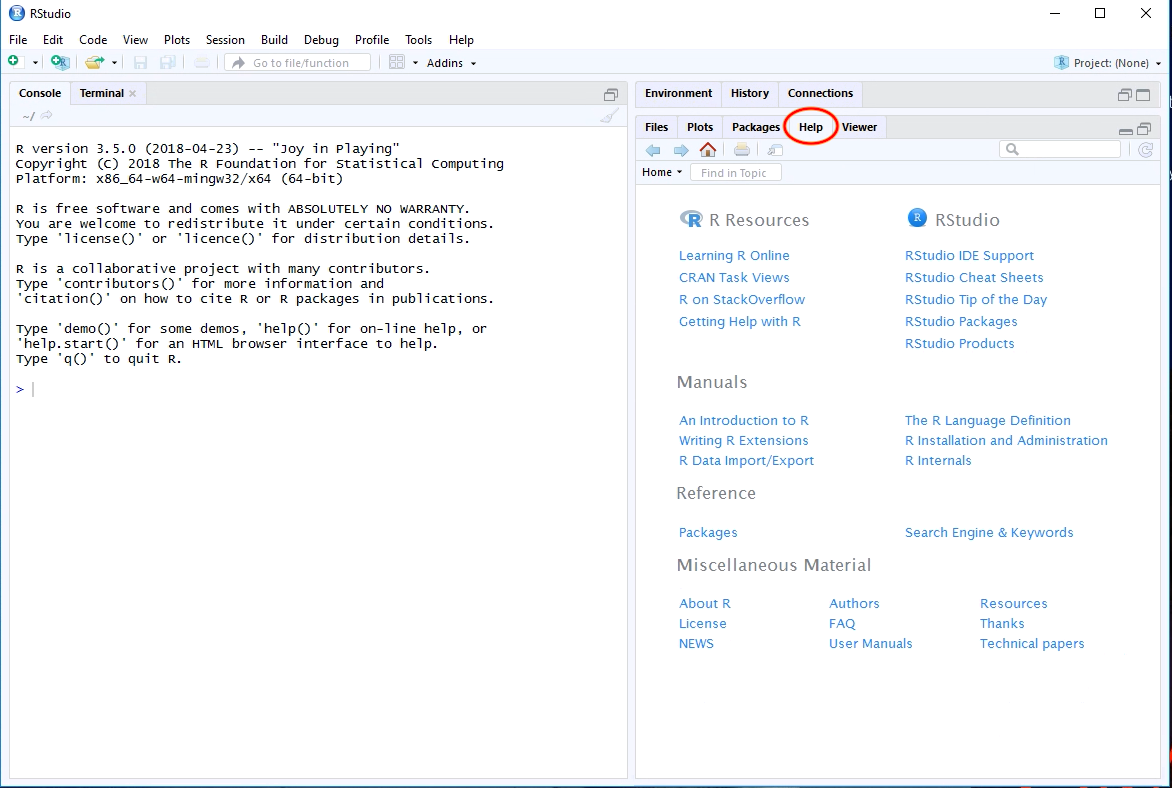
\includegraphics[width=\textwidth]{images/GH1.png}
        
        To get help on a specific package or function, simply type the name of that package or function in the search bar, and choose the correct item from the drop down menu. 
        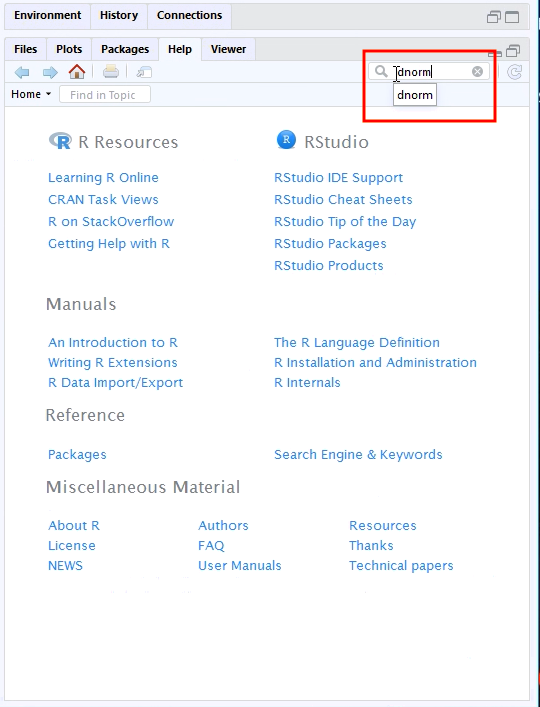
\includegraphics[width=\textwidth]{images/GH3.png}
        
       \newpage  After clicking the correct item, a help page will appear in the ``Help" Window. 
        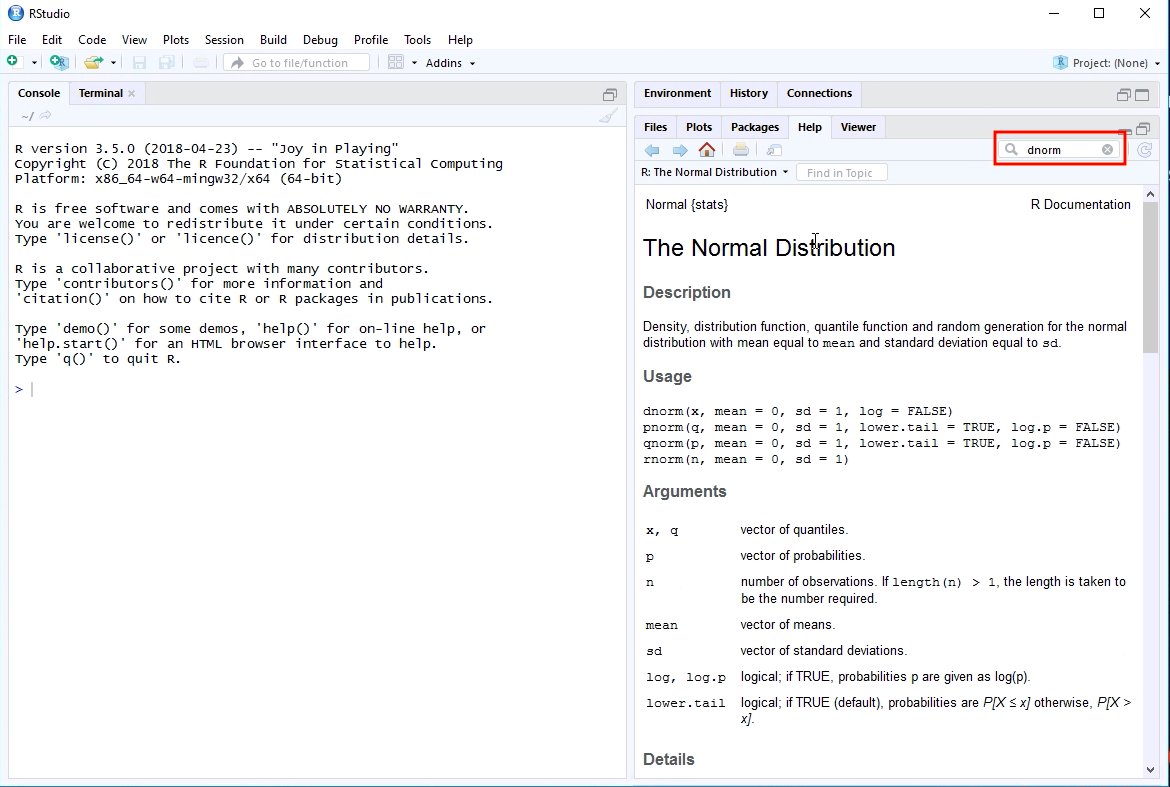
\includegraphics[width=\textwidth]{images/GH2.png}

        You can also type the following commands in the Console Window ``?dnorm" or ``help(dnorm)" and the same info page will appear in the ``Help" pane. 
        \end{flushleft}
        
        
\newpage \section{A Sample Program}
        \begin{flushleft}
        To get a basic idea of how RStudio works, we will create a sample program. 
        \newline\newline
        \textbf{Step-1:} To open a new R Script, either go to File $\longrightarrow$ \textbf{New File} $\longrightarrow$ \textbf{R Script}, or click the ``New File" icon in the top left corner, you can also use keyboard commands \textbf{``CTRL+SHIFT+N"} 
       
        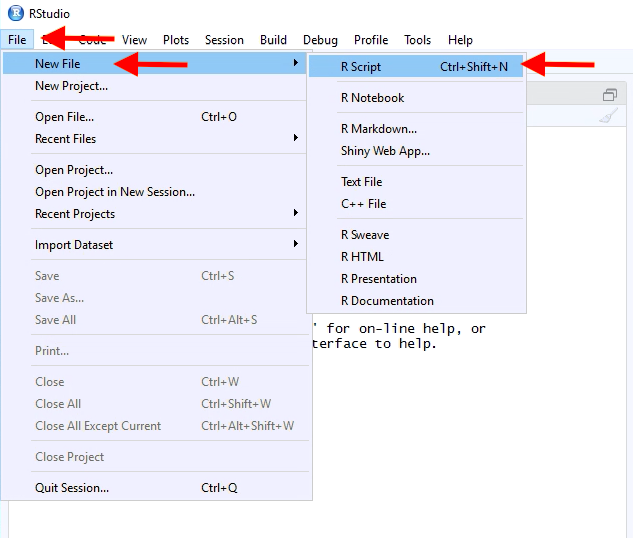
\includegraphics[width=4.2in, height = 4in]{images/SP1.png}
        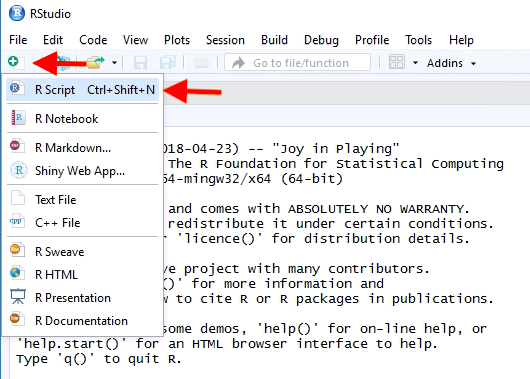
\includegraphics[width=3.7in, height = 3.6in]{images/SP2.png}
        
         \subsection*{Step 2-3}
        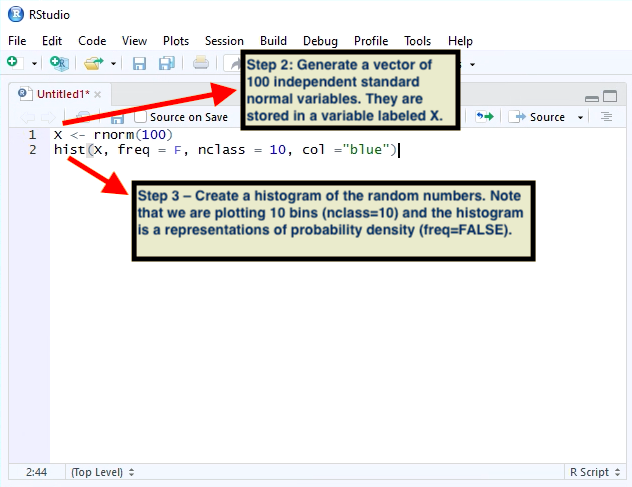
\includegraphics[width=5in, height = 4.2in]{images/SP3.png}
        
        \subsection*{Step 4}
        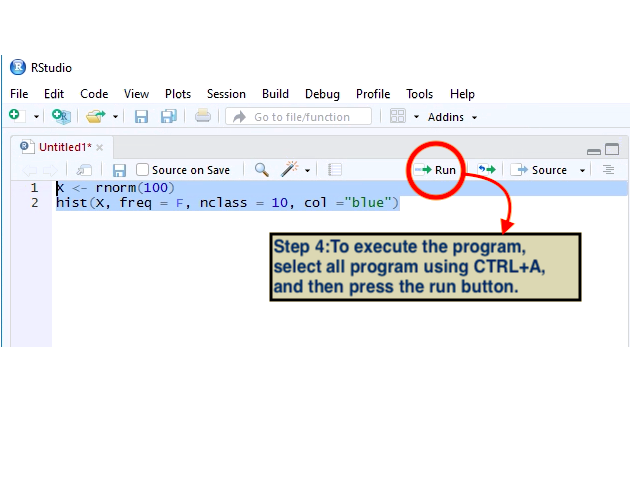
\includegraphics[width=5in, height = 3.6in]{images/SP4.png}
        
        \subsection*{Running a Program in RStudio}
        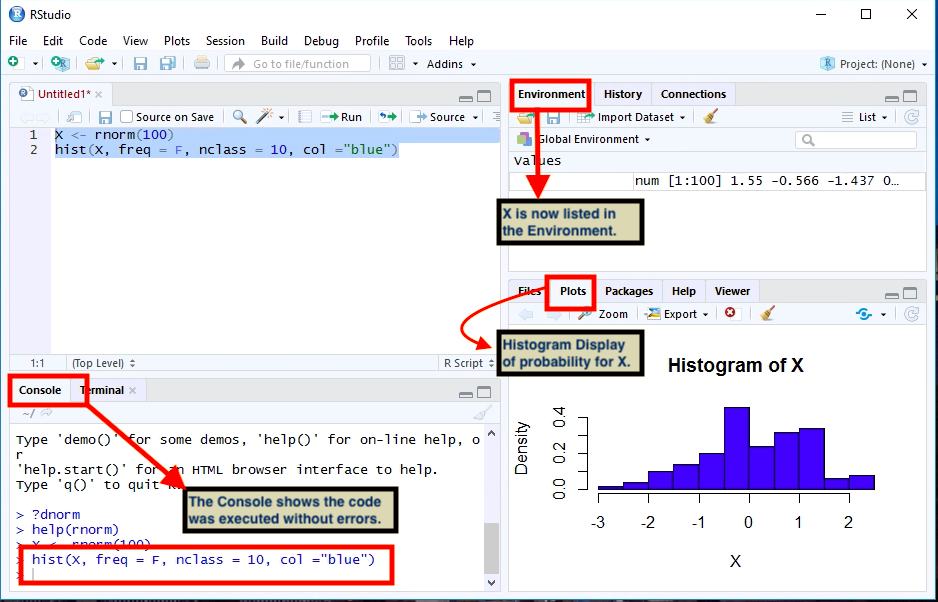
\includegraphics[width=\textwidth]{images/SP5.png}
        
        \subsection*{Step 5: Saving your script}
        To save the R script, either click on the Save icon  or from selecting the file menu: File $\longrightarrow$ \textbf{Save} as to have the Save as dialogue box. Select the directory that you want to store your project.
        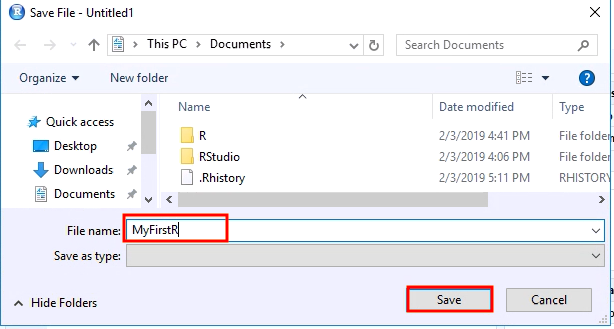
\includegraphics[width=\textwidth]{images/SP6.png}
        \end{flushleft}
    
    \section{Importing Data from an External Source}
    
        \begin{flushleft}
        It’s easy to input small size data set by typing, but for large datasets it’s always convenient to import them from the external source. For R, the easiest way to import and export data sets is using text files, however you can import data from various different sources including Excel, SAS, SPSS and Stata. 
        \newline\newline
        \textbf{Step 1} – Add a new Folder named “My R” in the location of My Documents. This is where we will save our dataset later.
        \newline \newline 
        \textbf{Step 2} - Open the ``PROFIT.txt'' data set from https://www.umbc.edu/circ/workshops/files/PROFIT.txt
        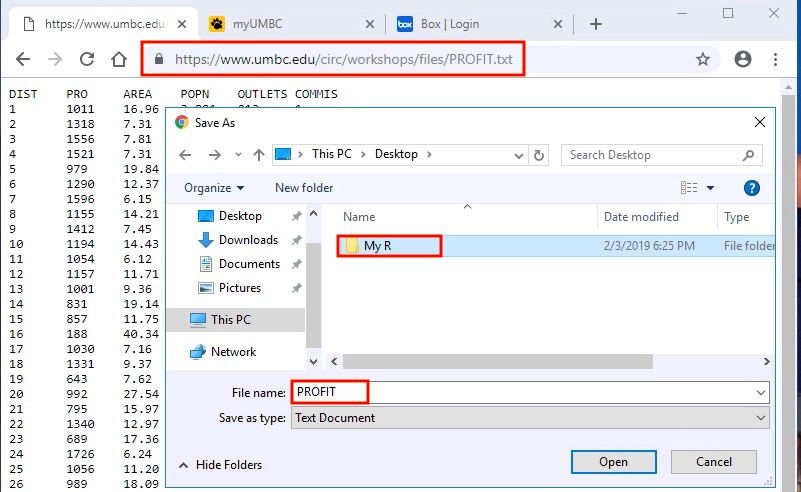
\includegraphics[width=\textwidth]{images/ID1.png}
        \newline\newline
        
        \textbf{Step 3} - Open RStudio, and display your current working directory typing ``getwd()'' in the R console:
        \newline \newline
        \textbf{Step 4} - Change the current working directory to your ``My R'' folder. 
        
        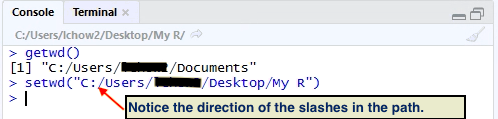
\includegraphics[width=\textwidth]{images/ID2.png}
        \newpage
        \textbf{Step 5} - Import from “PROFIT.txt” file into “mydata” in R by typing the command in the Editor window:
        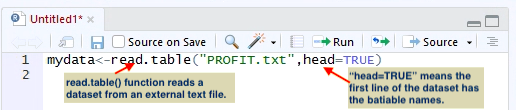
\includegraphics[width=\textwidth]{images/ID3.png}
        
        \textbf{**Note: R commands are case sensitive, so “mydata” and “MyData” are different objects.}
       \newline\newline
       
       \textbf{ Step 6} - Check whether your data set has been correctly imported: you can type the data set name in the R Console windows. Or in the ``Environment Window'' you can click the dataset's name and a new tab will appear in the area where the script pane is located. You can view the data here:
       \newline\newline
       
       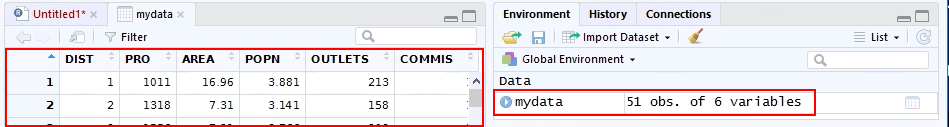
\includegraphics[width=\textwidth]{images/ID4.png}
           Thus, it shows the PROFIT.txt data has been successfully imported into R, and stored into a data frame named by “mydata”.
        \end{flushleft}
        
        
    \section{Exporting Data}
        \begin{flushleft}
        After we create and manipulate the original data, we may need to save the results. In RStudio, we can export the data set into text file using write.table ( ) function:
        
        The above command saved the file into the current working directory. If you want to save it to another directory, you need to indicate the full path.

       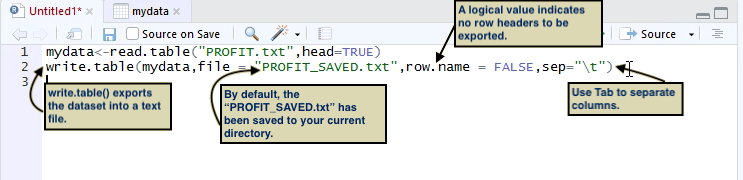
\includegraphics[width=\textwidth]{images/ID5.png}
       \end{flushleft}
 

\chapter{3 - Statistical Analysis Application}
        \begin{flushleft}
        The most important feature for RStudio is its applications in statistical analysis and related graphic display. There are various built-in functions for data analysis, and they are flexible and able to be customized. Through out the remainder of this workshop, we will use the PROFIT data set.
        \end{flushleft}
        
    \section{Creating a Histogram}
        \begin{flushleft}
        Histogram is a graph of the number of observations that fall within a specific range of values. It shows shape of the data distribution, e.g. normal, skewed right, skewed left, etc. To create a histogram of PRO variable in the PROFIT data, follow the steps as below (after each step, you need to press the ``Run'' button in the R Script Window tool bar to run it):
        \newline\newline
        \textbf{Step 1} - Add the data to the R search path to make the data set available to R by using the command ``attach(mydata)''. \textbf{(If you do not do this, you will have to reference the variables by indicating which dataset they are in with ``\$'' e.g. ``mydata\$PRO''.)}
        \newline\newline
        \textbf{Step 2} - Use hist( ) to plot the probability density of variable PRO:
        
        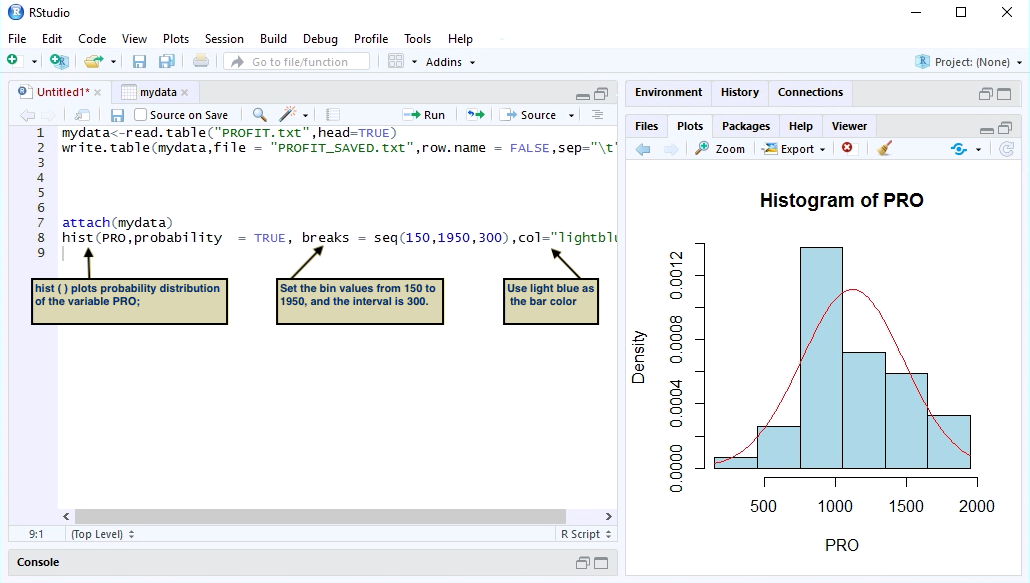
\includegraphics[width=5.5in,height=3.7in]{images/HIST1.png}
        
        \newpage
     \newpage  \textbf{Step 3} - Superimpose normal curve onto the histogram:
     
        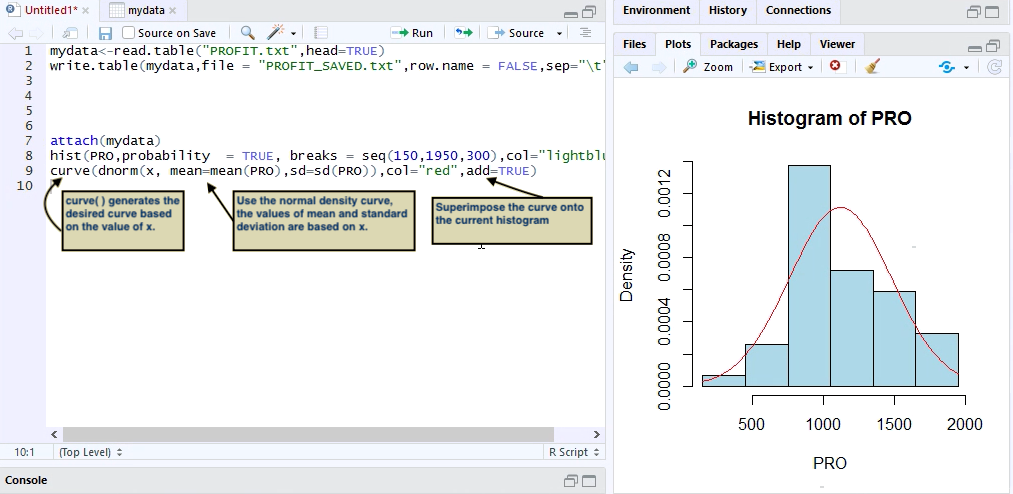
\includegraphics[width=\textwidth]{images/HIST2.png}
        \end{flushleft}
        
    \section{Creating a Scatter Plot}
        \begin{flushleft}
        Sometimes we are interested in the relationship between two variables in a dataset, rather than just the distribution of individual variable. Scatter plots can be used to answer the following questions:

        - Is their a relationship between X and Y linear? \newline
	    - Does the variation in Y change depending on X?
	    \newline
        - Are there any outliers?
        \newline
        Next, we use R to plot the two-dimensional scatter plots between Population add Profit to see how strong the relationship is between them. To create such a plot, use the command below: \newline \newline
        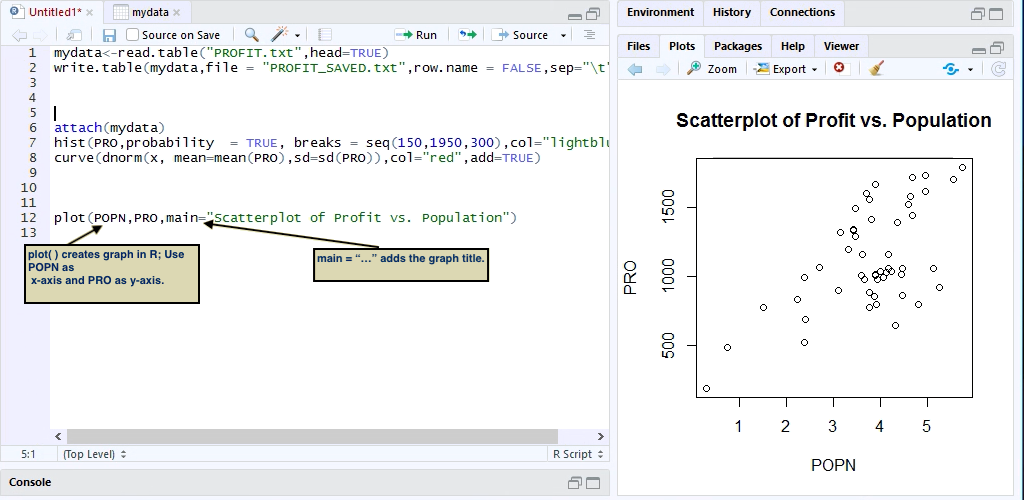
\includegraphics[width=\textwidth]{images/SCATTER1.png}

        \end{flushleft}
        
    \section{Computing Statistical Properties}
    
        \begin{flushleft}
        We can use statistical summary to summarize our observations. We can draw useful information from calculating the mean, median and standard deviation for further analysis. For the PROFIT data, we can use R to obtain it. Just add one command to the existing program: \begin{center}
            `` SUM=summary(mydata)''
        \end{center}
       
        We store the results into a variable called SUM, because it is necessary when we want to save the output. \newline 
        When it is done, run it, type SUM in the RStudio Console window. You should see the output in the Console Window. 
        \newline \newline
        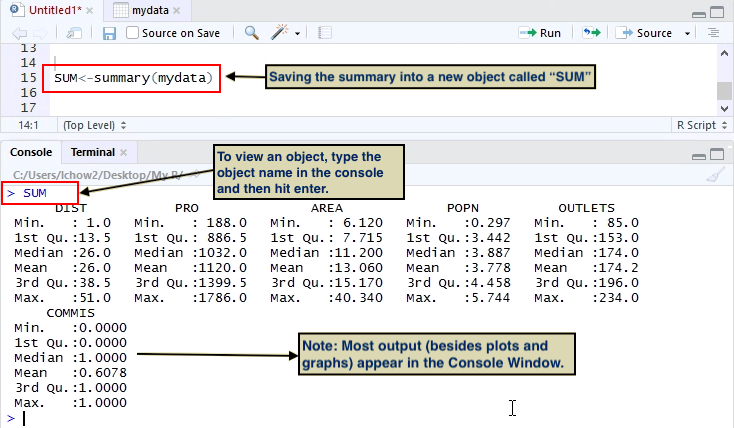
\includegraphics[width=\textwidth]{images/STATPROP1.png}
        \end{flushleft}
        
    \section{Hypothesis tests for the Mean}
    
        \begin{flushleft}
        From the histogram, we saw that the Profit variable was approximately centered around 900; however based on the above statistical summary we saw that the sample mean is 1120.0. We may be interested in the following hypothesis test:

        \textbf{Null Hypothesis ($H_{0}$):\hspace{0.5in}Mean of Profit $\leq$ 900 \newline
        Alternative Hypothesis ($H_{1}$):Mean of Profit $>$ 900}
        
        \newpage
        To test the hypothesis, use the following command below in the R Script window: \newline \newline

        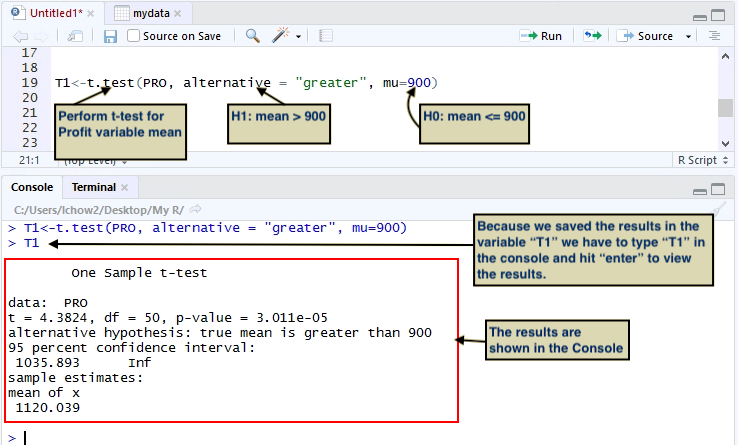
\includegraphics[width=\textwidth]{images/TTEST1.png}

        Since the P value is very small, we reject the null hypothesis and conclude that the mean of Profit variable is greater than 900 at 0.05 significant level.
        \end{flushleft}
        
    \section{Computing the Sample Correlations}
    
        \begin{flushleft}
        From the scatter plot, we saw that there exists a possible linear relationship between Profit and Population. To investigate the strength of such relationship, we can compute a sample correlation coefficient (r). r measures the degree of the linear relationship between two variables, and its range is [-1, 1]. The sign indicates the two variables are negatively or positively associated, and the absolute value measures the strength of the linear relationship. We can easily compute the value of sample correlation coefficient using R by the command:
        \begin{center}
           \textbf{ COR=cor(PRO,POPN)}
        \end{center}
        
                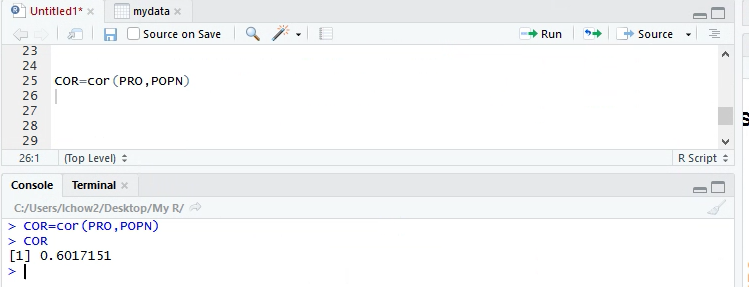
\includegraphics[width=5in,height=1.6in]{images/COR1.png}
        \end{flushleft}
        
    \section{Simple Linear Regression}
        \begin{flushleft}
        On the basis of the above analysis, we have found that between Profit and Population exist a fairly strong positive correlation. We may desire to predict the Profit for a known value of Population using a linear model. This purpose can be done a procedure called linear regression. In other words, we wish to fit a line to the data. This can be done in R using the command in the R Script Window:
        \newline \newline
        
        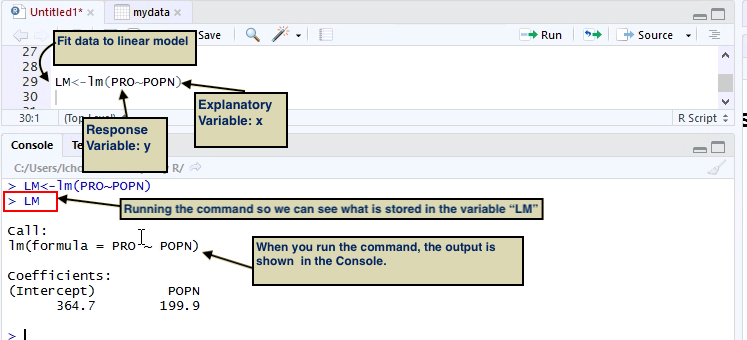
\includegraphics[width=\textwidth]{images/LM1.png}
        \newline \newline
        If you want to know more results from linear regression, you can simply enter ``LM\$'', then a drop down menu should appear showing you a list of available information. For example, \newline\newline 
        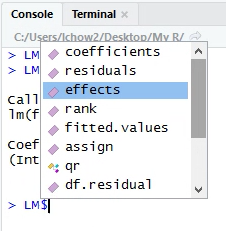
\includegraphics[width=2in,height=2.3in]{images/LM2.png}
        \newline
        You can check the detail information of each variable by typing its name (e.g. ``LM\$coefficients'')
        
        If there are multiple explanatory variables $x_{1}, x_{2}$ affecting the response variable $y$, you can perform multiple linear regression by using:\begin{center}
         \textbf{LM=lm(y$\sim$x1+x2)}
        \end{center}
    
        \end{flushleft}
        
    \section{Comparing Two Populations}
    
        \begin{flushleft}
        The PROFIT dataset contains a categorical variable called COMMIS with values 0 or 1. This variable identifies the commission area for the observation. We may be desired to compare the observations which have a COMMIS value of 0 vs. those with a value of 1. Using this categorical variable, we can compare the differences between groups. Box plot is one of the most useful graphic representations of such comparison. To create a Box Plot for Profit using COMMIS as a class variable in R, we can simply type the commands below:

         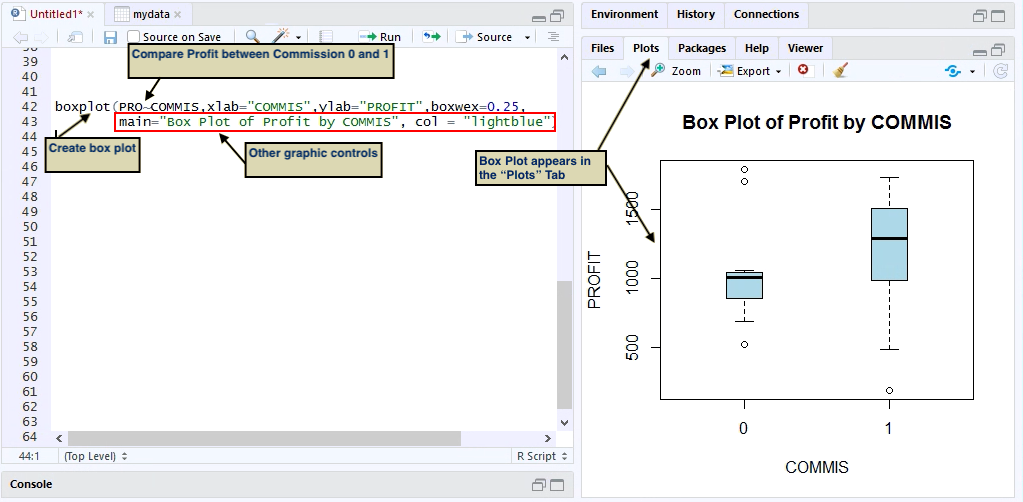
\includegraphics[width=\textwidth]{images/BXPLT1.png}
        \end{flushleft}
        
    \section{Two-Sample T-Test}
    
        \begin{flushleft}
        From above box plot we can see that the sample mean of each commission are not equal. Suppose we wish to be more objective in our analysis of the data, we can apply two-sample t-test to test the equality of the two population means. The appropriate hypothesis is: 
        \newline \newline
        \textbf{ $H_{0}$ (Null Hypothesis): \hspace{0.4in} Mean (COMMIS=0) $\geq$ Mean (COMMIS=1) \newline
        $H_{1}$ (Alternative Hypothesis): Mean (COMMIS=0) $<$ Mean (COMMIS=1)	}	
        \newpage
        In other words, we are interested in the test of the mean of Profit for COMMIS=1 is greater than that with COMMIS=0. In R, we can use the command below:
        (notice in the results the default level of significance is 0.05.)
        \newline\newline
         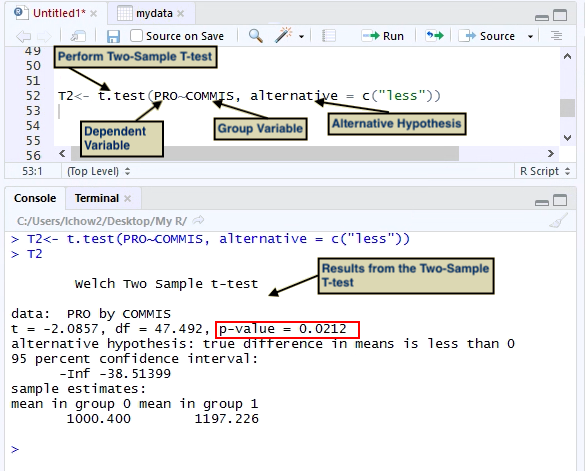
\includegraphics[width=\textwidth]{images/TTEST2.png}
         \newline \newline
         Because the P-Value is very small (0.0212), we reject the null hypothesis and conclude the Profit mean is significantly different between two commissions at the level of 0.05. This result is consistent with the box plot. 
        \end{flushleft}
        
        \newpage
        \section{Saving Your Project}
        \begin{flushleft}
            In RStudio, we can save each individual piece of our project including source code, graphics and the output. We will see how to save each of them using RStudio.
            \newline
            
            \textbf{Step 1}– Save R code. Go to the R Script window, and press the save icon in the tool bar. Then browse to your desired location to store the code, specify a name and click ``Save''. 
            
                    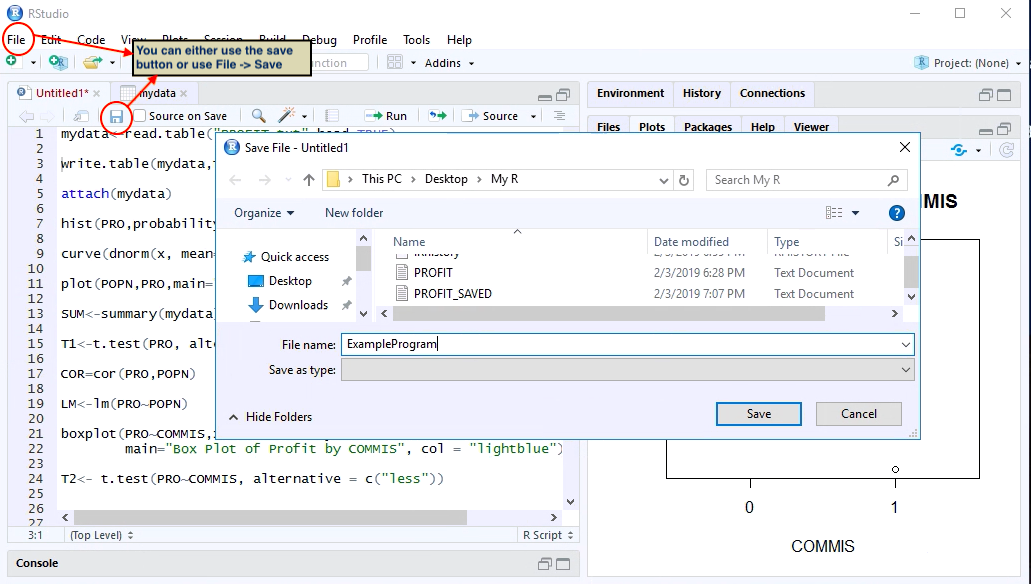
\includegraphics[width=\textwidth]{images/SAVE1.png}
            
            
            
            \textbf{Step 2} - Save the graphs by clicking the ``Export'' drop down menu in the ``Plots'' tab. Choose whether to export the plot or graph as a PDF or as an image. If you choose to export the plot or graph as an image you will be prompted to choose which file type you want to save the image as. 
            \newline \newline 
            
                    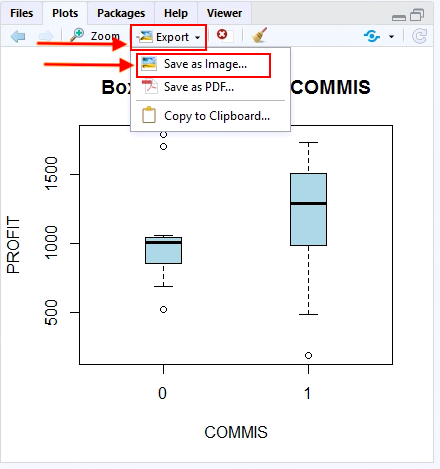
\includegraphics[width=2.40in,height=2.63in]{images/SAVE2.png}
                    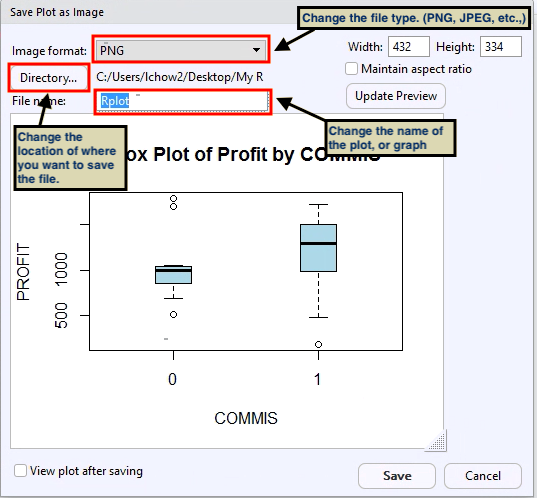
\includegraphics[width=2.63in,height=2.75in]{images/SAVE3.png}
    
            \textbf{Step 3} - Save the output as workspace. In R, we can save the output data as workspace file. To do this, go to the top menu bar, then select from the Session menu: Session$\longrightarrow$ \textbf{Save Workspace}. Then browse to save it to your desired location.
            \newline \newline
                    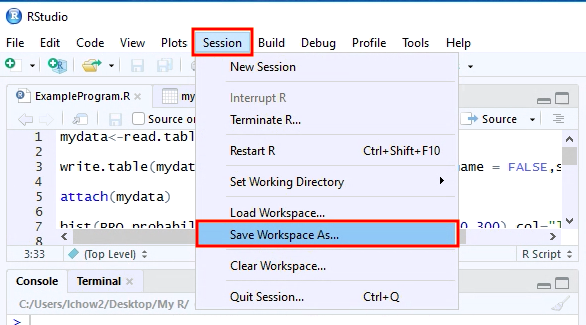
\includegraphics[width=\textwidth]{images/SAVE4.png}
                    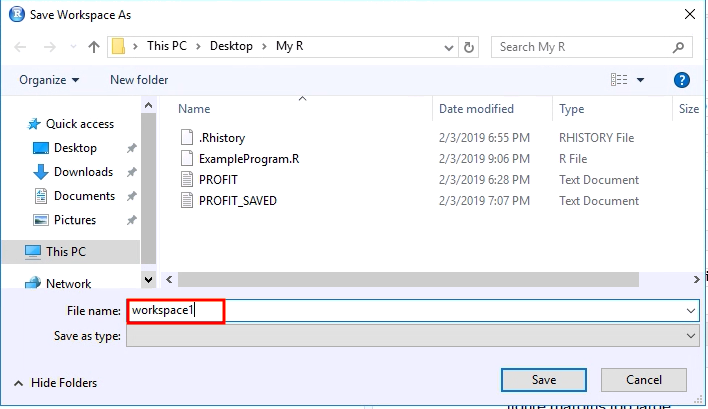
\includegraphics[width=\textwidth]{images/SAVE5.png}
                    
            \newpage
            
            When you open the workspace again by select: Session$\longrightarrow$ \textbf{Load Workspace}. 
            \newline \newline
                     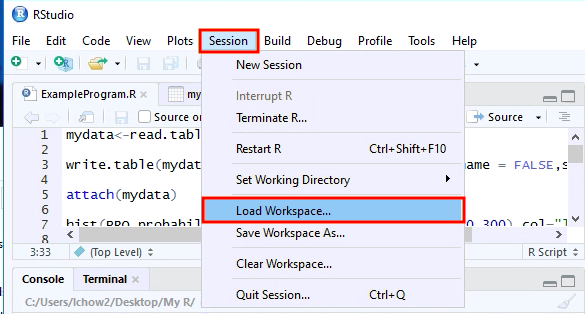
\includegraphics[width=5in,height=3in]{images/SAVE6.png}
            \newline \newline
            If you type ls( ) in the R Console window, we can see all the variable names in our source code. We can restore the outputs by typing the corresponding variable name, if you type COR, then the result of the correlation between Profit and Population variables will be restored.
            \newline\newline
                    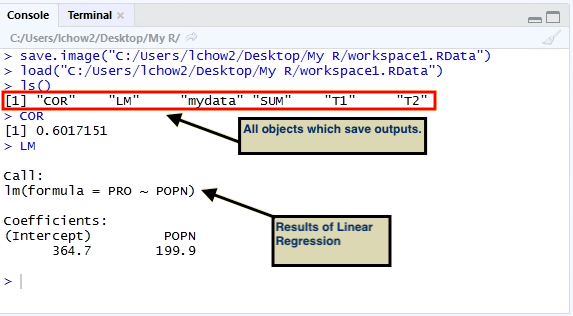
\includegraphics[width=5in,height=3in]{images/SAVE8.png}
        \end{flushleft}
      
    \newpage  \section{R Packages}
        \begin{flushleft}
        
        All functions in R are collected in packages. R comes with its base libraries. You can see the complete list of packages in your system by going to the pane \textbf{packages}. 
        \newline \newline 
                    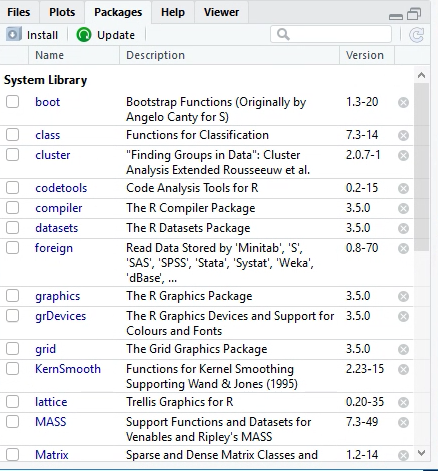
\includegraphics[width=3in,height = 3.5in]{images/PCK1.png}
      \newline  
        To install packages, activate the pane \textbf{packages}. Enter the first few letters from the name of the package. RStudio will list the package(s) starting with those letters. Select the package to be loaded from the list, if the package is not already installed, click on the install button and a dialog box will appear to walk you through the steps to install. Once installed, it will appear in this list to be loaded (or checked off).
        
                    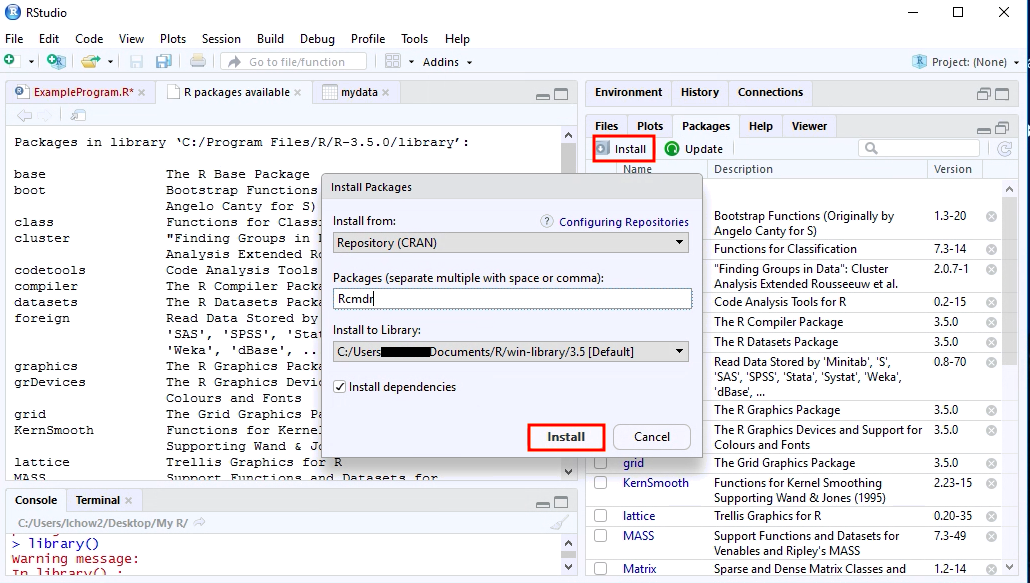
\includegraphics[width=4in,height=3.5in]{images/PCK2.png}

        
        Once the package is finished installing, go back to the pane \textbf{packages} and make sure it is checked off. When you check off a package from that list, it loads the package so that you can use its material (functions, datasets, etc.,) in your R Script. 
        
                    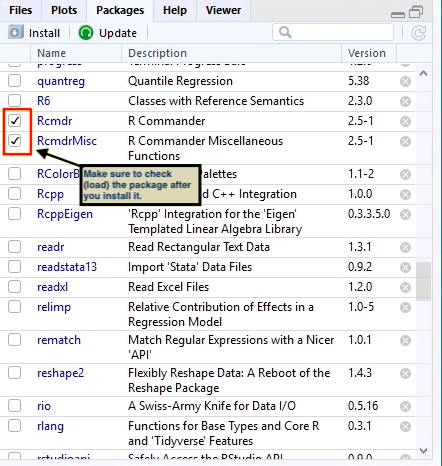
\includegraphics[width=3in,height=3.5in]{images/PCK3.png}

        \end{flushleft}

\end{document}
